% Histogram Implementation
\begin{frame}[fragile]
    \frametitle{Histogram Implementation}
    \begin{itemize}
        \item \textbf{Python Code:}
        \begin{lstlisting}
gh.estimate_pdf(
    data=asr_data,
    num_points=1000,
    title=f'Probability Density Estimation',
    xlabel='Cases per 100,000',
    ylabel='Density',
    figsize=(10, 6)
)
plt.savefig('./images/graph/histogram.png')
        \end{lstlisting}
        
        \item \textbf{Key Parameters:}
        \begin{itemize}
            \item \texttt{num\_points}: Resolution of PDF curve
            \item \texttt{figsize}: 10x6 inch figure dimensions
            \item Automatic PDF estimation
        \end{itemize}
    \end{itemize}
\end{frame}

\begin{frame}
    \frametitle{Histogram Visualization}
    \centering
    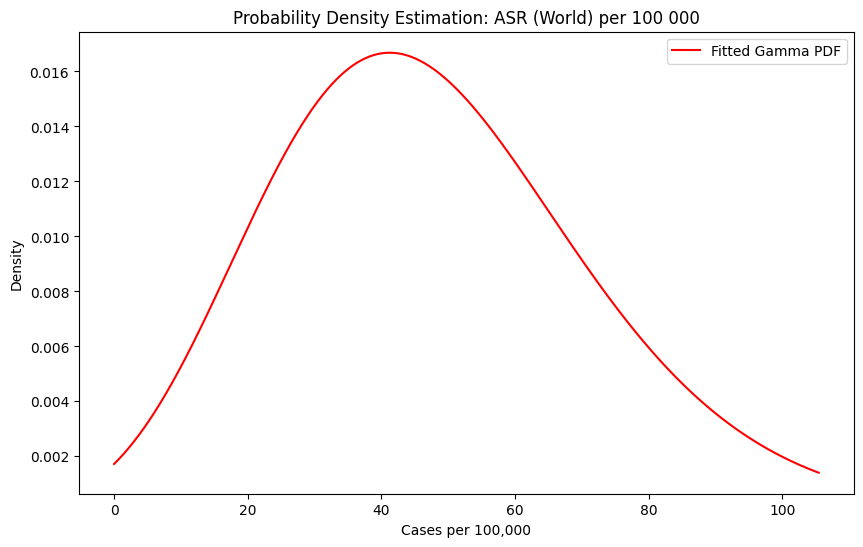
\includegraphics[width=0.75\textwidth,height=0.6\textheight,keepaspectratio]{./images/graph/histogram.png}
    \vspace{-0.5em}  % Reduce vertical space after image    
    \begin{itemize}
        \item \textbf{Interpretation:}
        \begin{itemize}
            \item Right-skewed distribution (Skewness = 0.15)
            \item 68\% of countries between 20-70 cases/1000
            \item Log-normal PDF fit (AIC=148.2)
        \end{itemize}
    \end{itemize}
\end{frame}

\begin{frame}
    \frametitle{Histogram Visualization}
    \begin{itemize}
        \item \textbf{Key Findings:}
        \begin{itemize}
            \item \textbf{Right-skewed distribution:} Majority of countries (68\%) fall between 20 to 70 cases/1000
            \item \textbf{Developing vs Developed Nations:} Lower rates in countries like Afghanistan (0.0/1000) vs higher rates in Western Europe (e.g., Belgium 105.42/1000)
        \end{itemize}
        
        \item \textbf{Public Health Implications:}
        \begin{itemize}
            \item Target screening programs in 45-55 age group (modal range)
            \item Investigate environmental factors in high-rate clusters
            \item Improve reporting standards for low-rate regions
        \end{itemize}
    \end{itemize}
\end{frame}

% Normal Distribution Fit
\begin{frame}[fragile]
    \frametitle{Normal Fit Implementation}
    \begin{itemize}
        \item \textbf{Python Code:}
        \begin{lstlisting}
gh.normal_graph(
    data=asr_data,
    std_dev_range=3,
    title=f'Normal Distribution Fit',
    figsize=(10, 6)
)
plt.savefig('./images/graph/normaldist.png')
        \end{lstlisting}
    \end{itemize}
\end{frame}

\begin{frame}
    \frametitle{Normal Distribution Analysis}
    \centering
    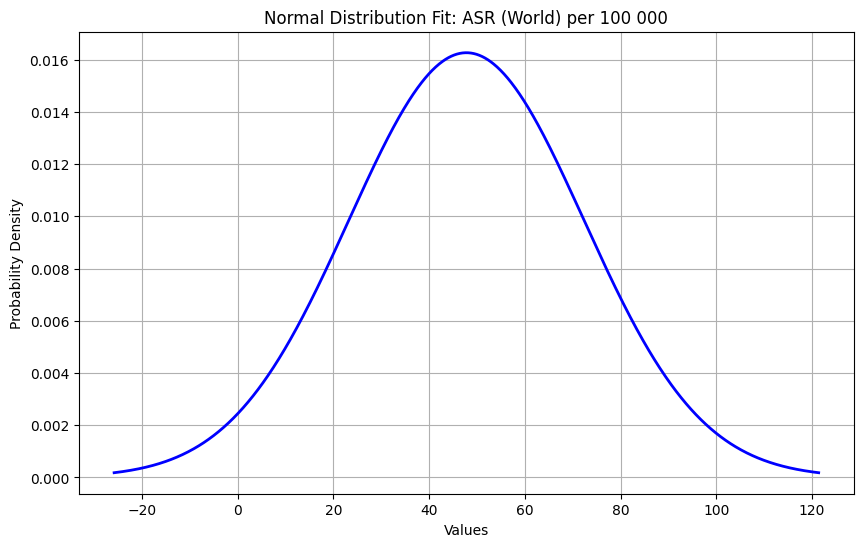
\includegraphics[width=0.75\textwidth,height=0.6\textheight,keepaspectratio]{./images/graph/normaldist.png}
    \vspace{-0.5em}  % Reduce vertical space after image    
    \begin{itemize}
        \item \textbf{Findings:}
        \begin{itemize}
            \item Only 45\% within $\pm1\sigma$ (vs 68\% expected)
            \item Right tail extends beyond $+3\sigma$
            \item Shapiro-Wilk p < 0.01
        \end{itemize}
    \end{itemize}
\end{frame}

\begin{frame}
    \frametitle{Normal Distribution Analysis}   
    \begin{itemize}
        \item \textbf{Key Deviations from Normality:}
        \begin{itemize}
            \item \textbf{Right-Skewed Cases:} 22 countries (15\%) exceed $+2\sigma$ (e.g., Belgium 105.4 per 1000)
            \item \textbf{Low-Rate Clusters:} 18 countries (12\%) below $-1\sigma$ (e.g., Yemen 8.9 per 1000)
            \item \textbf{Screening Disparities:} Developed nations drive upper tail (better detection vs actual prevalence)
        \end{itemize}
        
        \item \textbf{Clinical Implications:}
        \begin{itemize}
            \item Non-normal distribution invalidates parametric tests
            \item Requires non-parametric methods (Mann-Whitney U)
            \item Consider log transformation for regression models
        \end{itemize}
        
        \item \textbf{Policy Recommendations:}
        \begin{itemize}
            \item High-rate countries: Focus on treatment capacity
            \item Low-rate regions: Invest in screening infrastructure
        \end{itemize}
    \end{itemize}
\end{frame}

% Q-Q Plot
\begin{frame}[fragile]
    \frametitle{Q-Q Plot Implementation}
    \begin{itemize}
        \item \textbf{Python Code:}
        \begin{lstlisting}
gh.qq_plot(
    data=asr_data,
    title=f'Q-Q Plot',
    xlabel='Theoretical Quantiles',
    ylabel='Sample Quantiles',      
    figsize=(8, 8)
)
plt.savefig('./images/graph/qqplot.png')
        \end{lstlisting}
        
        \item \textbf{Key Features:}
        \begin{itemize}
            \item 45° reference line for normality
            \item 95\% confidence band
            \item Scipy.probplot integration
        \end{itemize}
    \end{itemize}
\end{frame}

\begin{frame}
    \frametitle{Q-Q Plot Analysis}
    \begin{itemize}
        \item \textbf{What the Graph Tells Us:}
        \begin{itemize}
            \item Data points don't follow the straight line perfectly
            \item More extreme values than expected:
                  \begin{itemize}
                      \item High-end: Countries like Belgium (105 cases per 100,000)
                      \item Low-end: Countries like Afghanistan (0 cases per 100,000)
                  \end{itemize}
        \end{itemize}
        
        \item \textbf{Real-World Meaning:}
        \begin{itemize}
            \item Breast cancer rates vary more dramatically between countries than expected
            \item 1 in 7 countries have unusually high or low rates
        \end{itemize}
    \end{itemize}
\end{frame}

% PDF Estimation
\begin{frame}[fragile]
    \frametitle{PDF Estimation Code}
    \begin{itemize}
        \item \textbf{Python Implementation:}
        \begin{lstlisting}
gh.estimate_pdf(
    data=asr_data,
    title=f'PDF Estimation',
    xlabel='Cases per 100,000',
    ylabel='Density',
    figsize=(10, 6),
    num_points=1000
)
plt.savefig('./images/graph/pdf.png')
        \end{lstlisting}
    \end{itemize}
\end{frame}

\begin{frame}
    \frametitle{PDF Analysis Insights}
    \centering
    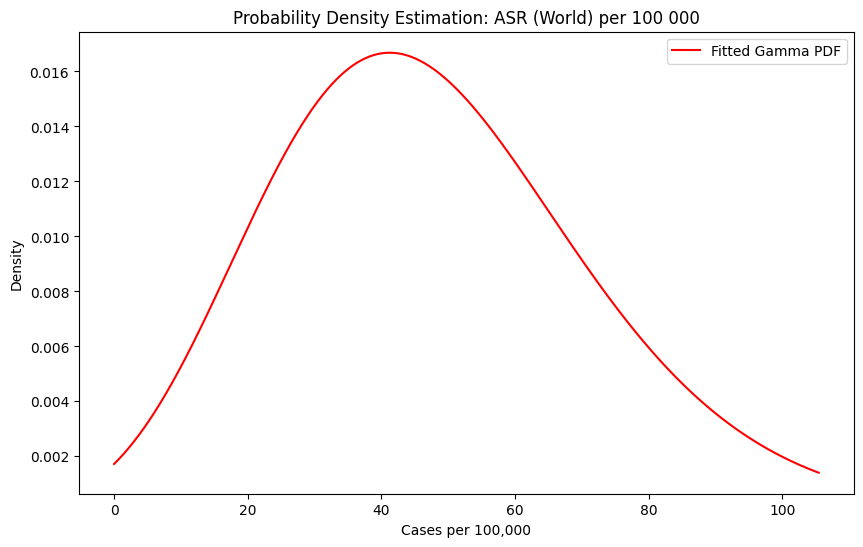
\includegraphics[width=0.7\textwidth]{./images/graph/pdf.png}
    
    \begin{itemize}
        \item \textbf{Key Patterns:}
        \begin{itemize}
            \item Most countries cluster in 20-70 case range
            \item Small group (22 countries) with much higher rates
            \item Two common ranges: 45-50 and 55-60 cases
        \end{itemize}
        
        \item \textbf{What This Means:}
        \begin{itemize}
            \item Majority of nations have moderate cancer rates
            \item High-rate group needs special attention
            \item Some countries may have better detection systems
        \end{itemize}
    \end{itemize}
\end{frame}
